\documentclass[letter]{ieice}
\usepackage[ruled,linesnumbered]{algorithm2e}
\usepackage{amssymb,amsthm,amsmath}
\usepackage{balance}
\usepackage{graphicx}          % graphicx package for including ps files  
\usepackage{epsfig}
\usepackage{url}
\usepackage{subfigure}
\usepackage{algorithmic}
\usepackage{float}
\newtheorem{theorem}{Theorem}[section]
\newtheorem{lemma}[theorem]{Lemma}
\usepackage{latexsym}
\usepackage{multirow}
\usepackage{color}
\usepackage{url}
\usepackage{comment}
%\usepackage{pstricks}
\usepackage{array}
\usepackage{epstopdf}
\newcolumntype{L}[1]{>{\raggedright\let\newline\\\arraybackslash\hspace{0pt}}m{#1}}
\newcolumntype{C}[1]{>{\centering\let\newline\\\arraybackslash\hspace{0pt}}m{#1}}
\newcolumntype{R}[1]{>{\raggedleft\let\newline\\\arraybackslash\hspace{0pt}}m{#1}}

\setcounter{page}{1}
%\breakauthorline{}% breaks lines after the n-th author

\field{D}
\title{SEDONA: A Novel Protocol for Identifying Infrequent, Long-Running Daemons on a Linux System}
%\titlenote{This work was in part supported by the EDISON program (NRF-2011-0020576).}
\authorlist{
 \authorentry[yksuh@kisti.re.kr]{Young-Kyoon SUH}{m}{labelA}
 %\authorentry[rts@cs.arizona.edu]{Richard T. Snodgrass}{n}{labelB}}
\affiliate[labelA]{Supercomputing R\&{D} Center, KISTI, 245 Daehangno, Yuseong-gu, Daejeon, 34141, Republic of Korea}
%\affiliate[labelB]{Department of Computer Science, University of Arizona, Tucson, AZ 85721, USA}
}
\received{2017}{2}{28}

\definecolor{grey}{RGB}{200,200,200}
\newcommand{\hilite}[1]{\colorbox{grey}{#1}}
\newcommand{\hilitey}[1]{\colorbox{yellow}{#1}}
\newcommand{\hiliting}[1]{\colorbox{grey}{#1}}
\long\def\todo#1{\hilitey{{\bf TODO:} {\em #1}}}
\long\def\shorten#1{}
\long\def\comment#1{}

\begin{document}

\maketitle

\begin{summary}
%It is challenging to accurately measure the execution-time of a given
%program due to many extraneous factors. To enable better timing results\shorten{restrained},
%we present a novel protocol that identifies infrequent, 
%long-running daemons to enable effective elimination of executions 
%exhibiting these daemons.
{\color{blue}Measuring program execution time 
a \hbox{much-used} technique for performance evaluation in computer science. 
Without a proper care, however, timed results may vary a lot, 
thus making it hard to trust their validity. 
In this paper we propose a novel timing protocol to significantly 
reduce such variability.}

\end{summary}
\begin{keywords}
Infrequent Long-running Daemon, Execution-Time Measurement
\end{keywords}

\section{Introduction}
\label{sec:intro}

Measuring program execution time is a much-used
technique for performance evaluation in computer science. 
Despite the importance of accurate and precise execution-time measurement, 
how to achieve {\em better} timing has not been well addressed. 
{\color{blue} Surprisingly, there is considerable variability in the measured time.
%which indeed suggests the need for a better timing protocol.
The goal of this paper is to propose
a better timing protocol that can significantly reduce such variability 
and thus enable better timing results without a doubt of their validity.}

Consider a simple compute-bound program, what we term {\em PUT} (program-under-test), 
as shown in Fig.~\ref{alg:put}. 
This program runs a nested for-loop with a specified task length ($tl$) (in seconds). 
%The $tl$ value is translated to the corresponding 
%number of {\color{blue}repetitions} for which that for-loop is performed. 
{\color{blue}The $tl$ value is used to compute 
the number of repetitions ($t$) for which that for-loop is performed 
to reach the specified task length.}

\vspace{-.2in}
\begin{figure}[h]
\begin{center}
\begin{algorithmic}
{\bf Algorithm} PerformManyIncrements($tl$): \\
\STATE $t$ = $tl$ * {CONSTANT} \\
\FOR{$k$ = 1 to $t$ by 1}
	\FOR{$i$ = 1 to {UINT\_MAX}-1 by 1}
		\STATE $j$ += 1 \\
	\ENDFOR 
\ENDFOR 
\end{algorithmic}
\end{center}
\caption{Computation by a Program-Under-Test (PUT)\label{alg:put}}
\vspace{-.2in}
\end{figure}

We used 128~seconds as the task length and ran the PUT program (termed PUT128) 
800~times. 
%Fig.~\ref{fig:meas_comp} shows two histograms of the timing results on PUT128.
{\color{blue}Fig.~\ref{fig:meas_comp} shows two plots of the timing results on PUT128.
%Most of the 800 repetitions measured in elapsed time, 
%via  {\tt System.currentTimeMillis()} in Java, are gathered in the tallest bar 
%of \hbox{128,000--129,000 msec,} with just a few executions outside of that bar, 
%as can be seen in Fig.~\ref{fig:hist_before_et}. 
Most of the 800 repetitions measured in elapsed time, 
via  {\tt System.currentTimeMillis()} in Java, form the central band 
of \hbox{128,000--129,000 ms,} as can be seen in Fig.~\ref{fig:hist_before_et}. 
There also exist over a dozen of repetitions above that band, called outliers.
But these outliers {\em critically} impact the overall measurement quality: 
a standard deviation of 1,730 ms and a relative error of 0.01.
This result suggests adequately eliminating these outliers 
while retaining most of the measured executions.}

{\color{blue}
Our protocol, which we propose shortly, on the contrary, 
effectively identifies and removes those outliers. 
In effect, the protocol considerably reduces such variability.
The protocol identified and removed fifteen repetitions 
that had {\em infrequent, \hbox{long-running} daemon processes}, 
impacting the execution time of PUT128. 
In addition, the protocol utilized {\em process time} (PT) (of PUT128) 
rather than elapsed time (ET). 
Using PT is preferred, in that it considers 
the time taken for only a process of interest.
PT can be calculated as the sum of ticks (where one tick is equal to 10 msec)
in user and system mode, available via {\tt taskstats} C struct, 
provided by the Linux NetLink facility~\cite{Netlink}.
As a result, none of the retained timing results was outside of 
the central band in Fig.~\ref{fig:hist_after_pt}, and thus 
the measurement quality---in both standard deviation and relative error---was 
improved up to by three orders of magnitude for PUT128, 
as shown in Fig.~\ref{fig:hist_after_pt}.
}

%The key idea to the protocol is to (i)~utilize
%{\em process time} (PT) rather than on elapsed time (ET) and 
%(ii)~throw out some executions that involve
%{\em infrequent, \hbox{long-running} daemon processes}, which impact
%the process time of the process. 
%Using PT is preferred, in that it considers 
%the time taken for only a process of interest.
%PT can be calculated as the sum of ticks (where one tick is equal to 10 msec)
%in user and system mode, available via {\tt taskstats} C struct, 
%provided by the Linux NetLink facility~\cite{Netlink}.
%This use of PT and selective elimination 
%was able to improve 
%measurement quality---in both standard deviation and relative error---up to by 
%three orders of magnitude for PUT128, as illustrated in Fig.~\ref{fig:hist_after_pt}. 
%}

%\vspace{0.05in}
{\bf Related Work.} 
McGeoch introduced
two basic methods of measuring program time: elapsed time and CPU time~\cite{Mcgeoch12}. 
Bryant and O'Hallaron~\cite{Randal03} 
presented two timing schemes of using clock-cycle and interval counters. 
They proposed a measurement protocol, called {\em minimum-of-k}, 
that for observed elapsed ticks the minimum is chosen as the most accurate one. 
Odom et al.'s work~\cite{Odom05} focused on timing long-running programs 
in a simulation framework via dynamic sampling of trace snippets during program execution. 
None of these prior works, however, takes into account the variability in 
timing and the influence of daemons that may significantly disturb the timing.

%\begin{figure}[t]
%	\centering
%	\subfigure[Initial Elapsed Time Measurement]{
%		%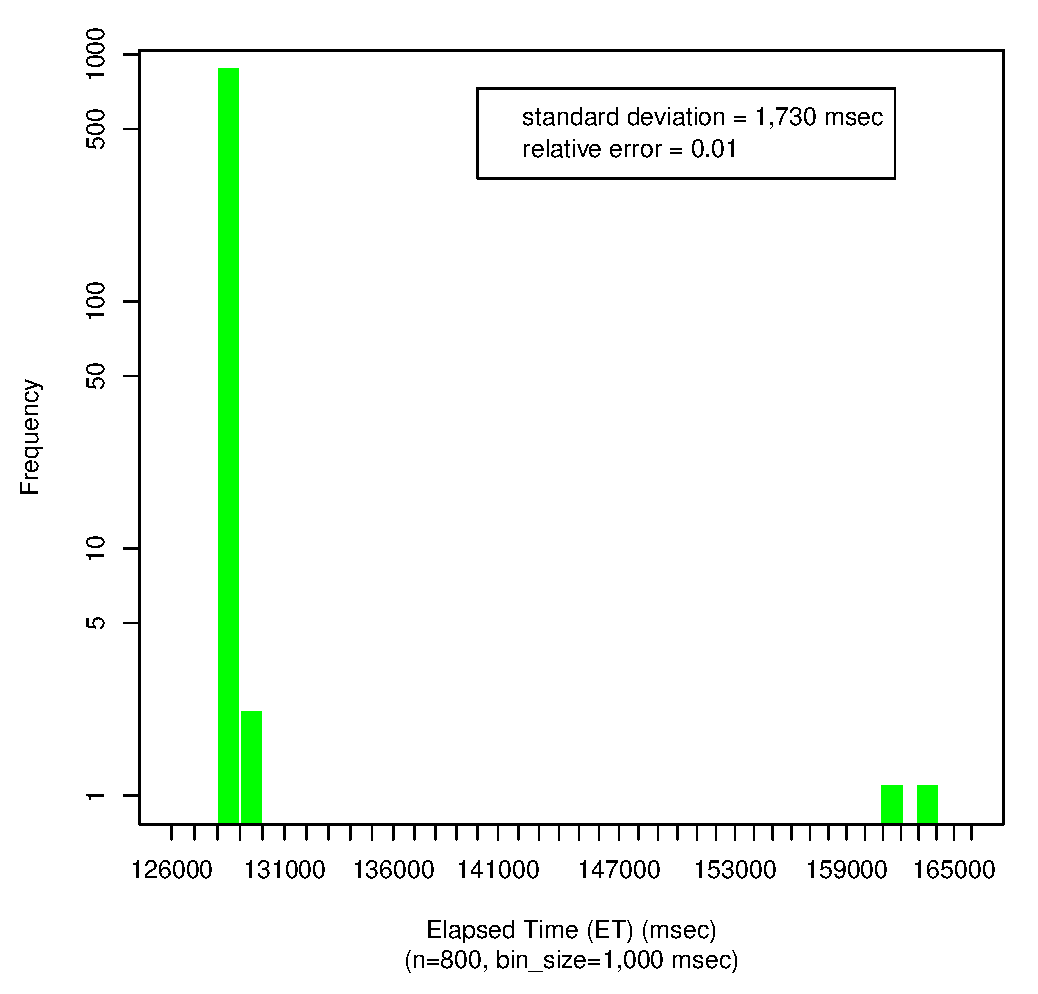
\includegraphics[width=0.31\textwidth]{128_sec_et_old_hist.eps}
%		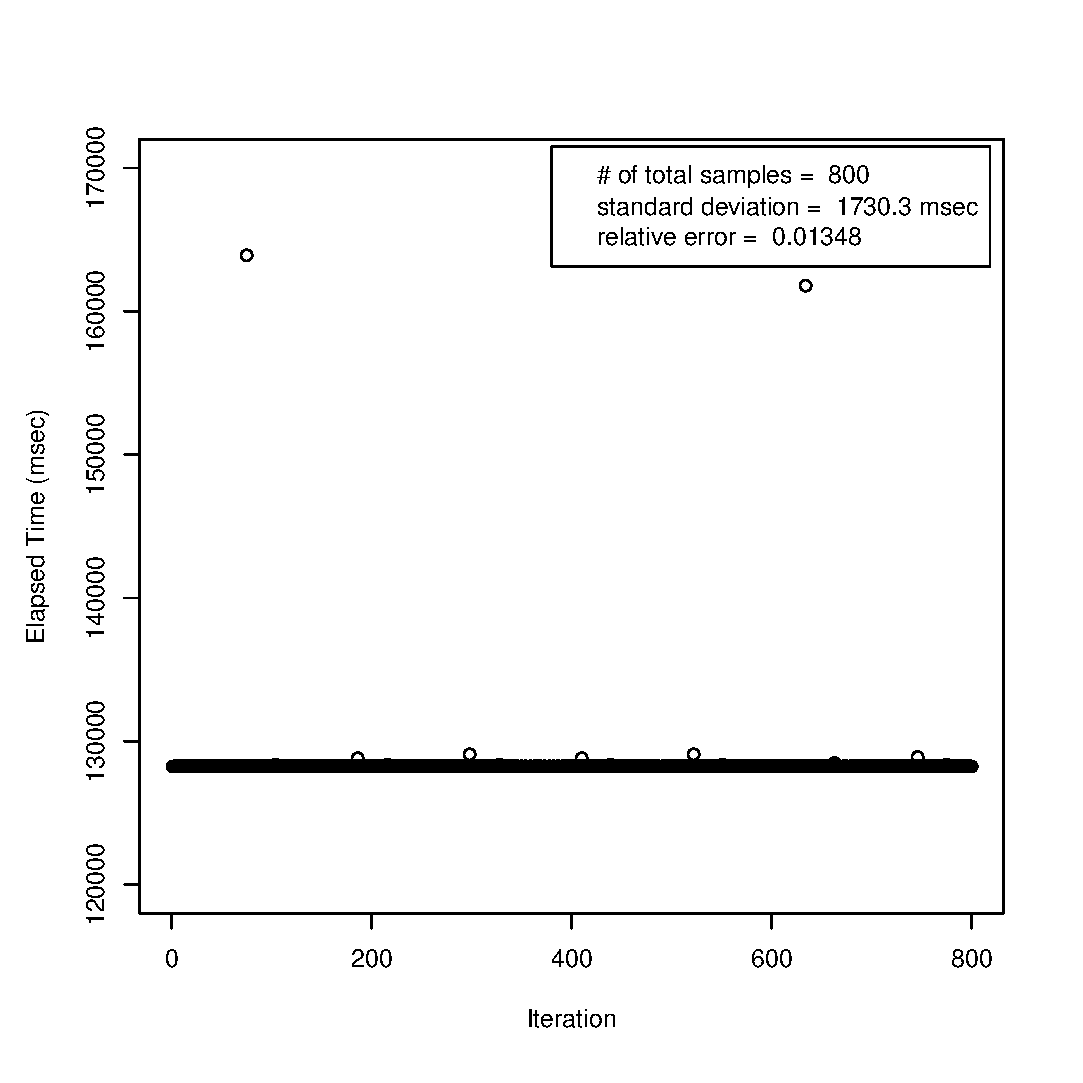
\includegraphics[width=0.31\textwidth]{128_sec_et_old.eps}
%		\label{fig:hist_before_et}
%	}
%	\subfigure[Program Time After Our Protocol]{
%		%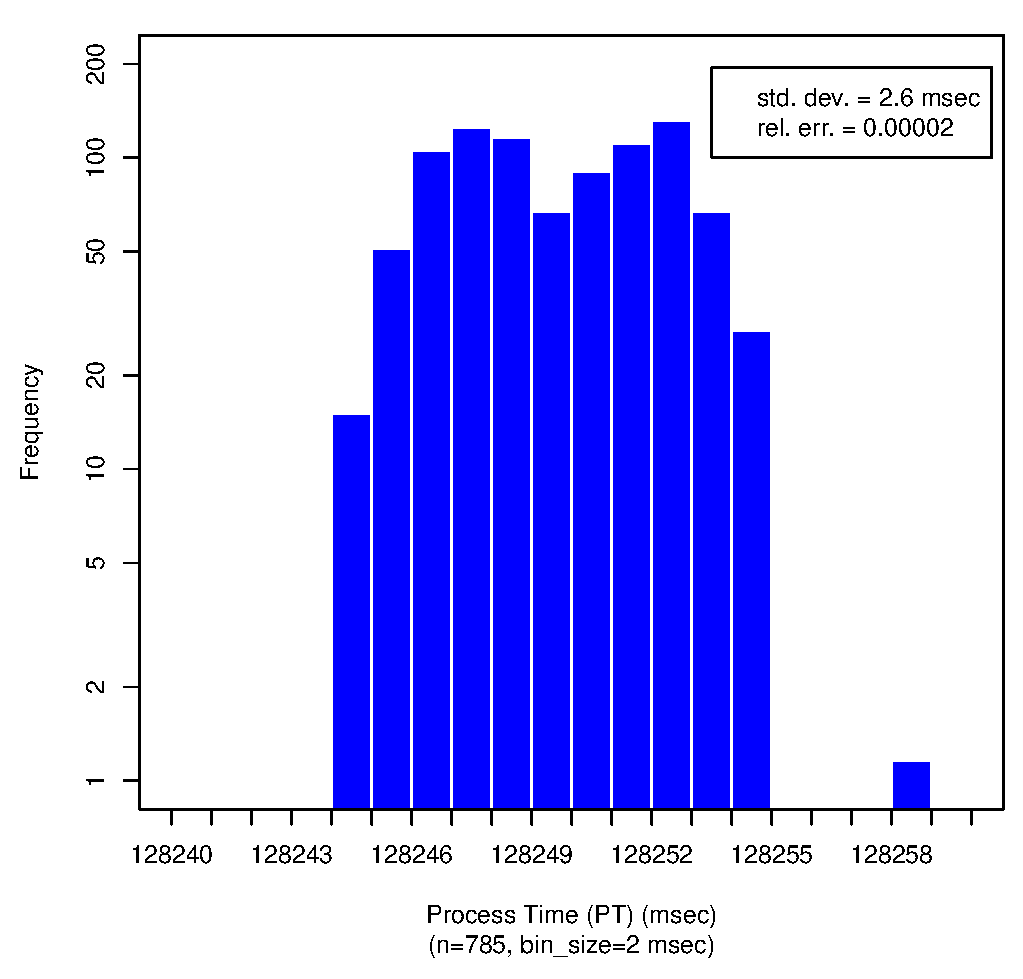
\includegraphics[width=0.31\textwidth]{128_sec_pt_new_hist.eps}
%		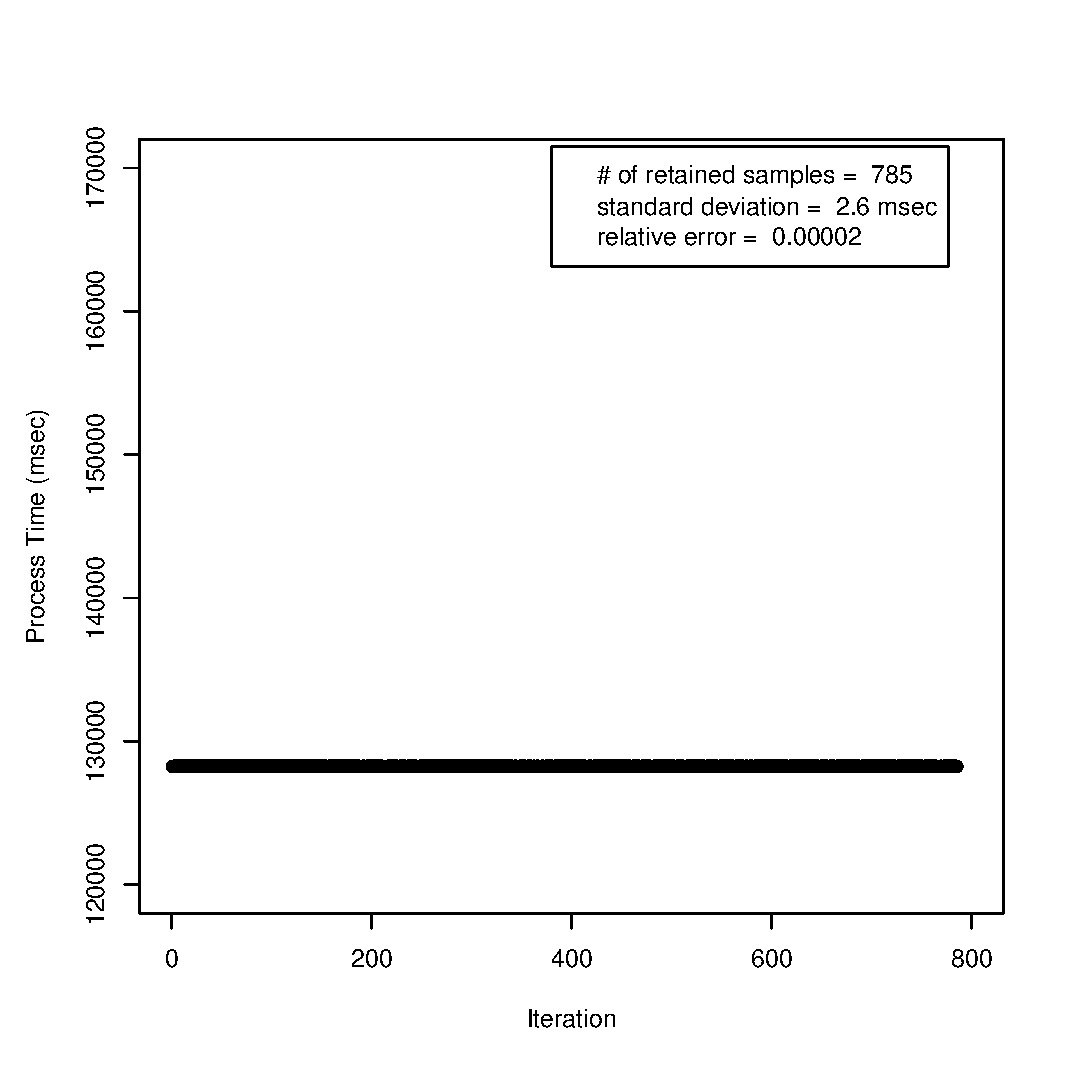
\includegraphics[width=0.31\textwidth]{128_sec_pt_new.eps}
%		\label{fig:hist_after_pt}
%	}
%	\caption{An Example of Measurement Results on a \linebreak \hbox{Compute-bound} 
%	Program-Under-Test~\label{fig:meas_comp}}
%	\vspace{-.18in}
%\end{figure} 

\begin{figure}[t]
	\centering
	\subfigure[Initial Elapsed Time Measurement]{
		%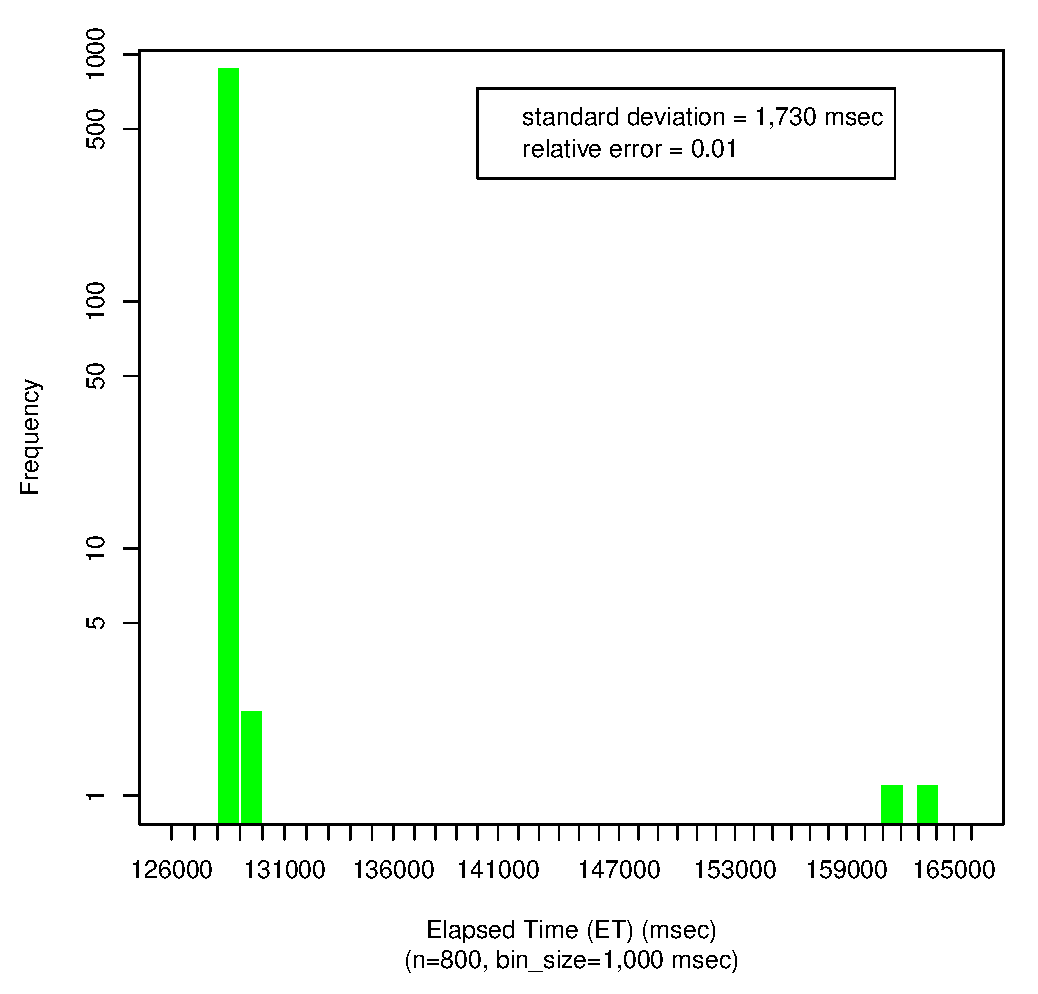
\includegraphics[width=0.31\textwidth]{128_sec_et_old_hist.eps}
		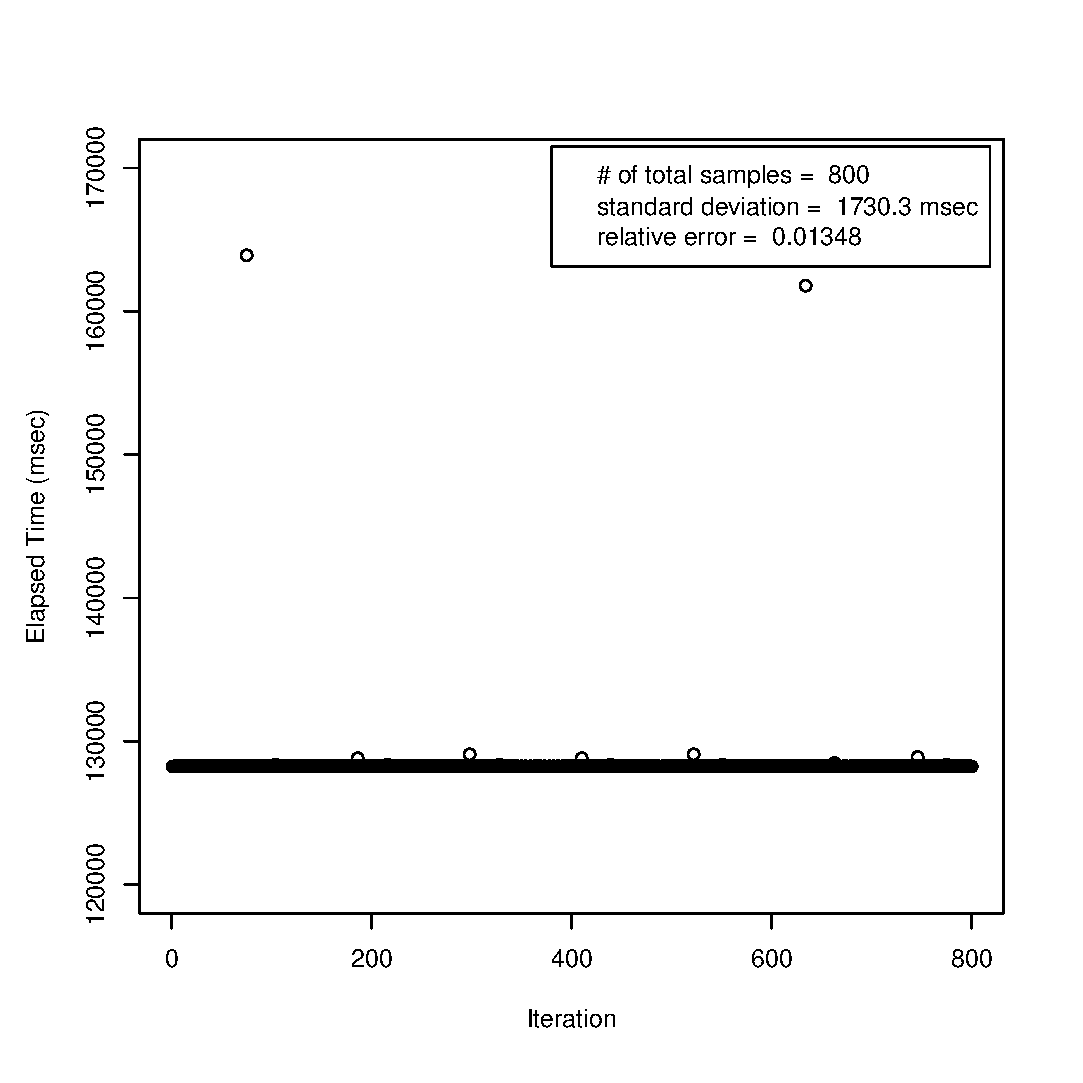
\includegraphics[width=0.224\textwidth]{128_sec_et_old.eps}
		\label{fig:hist_before_et}
	}
	\subfigure[Program Time After Our Protocol]{
		%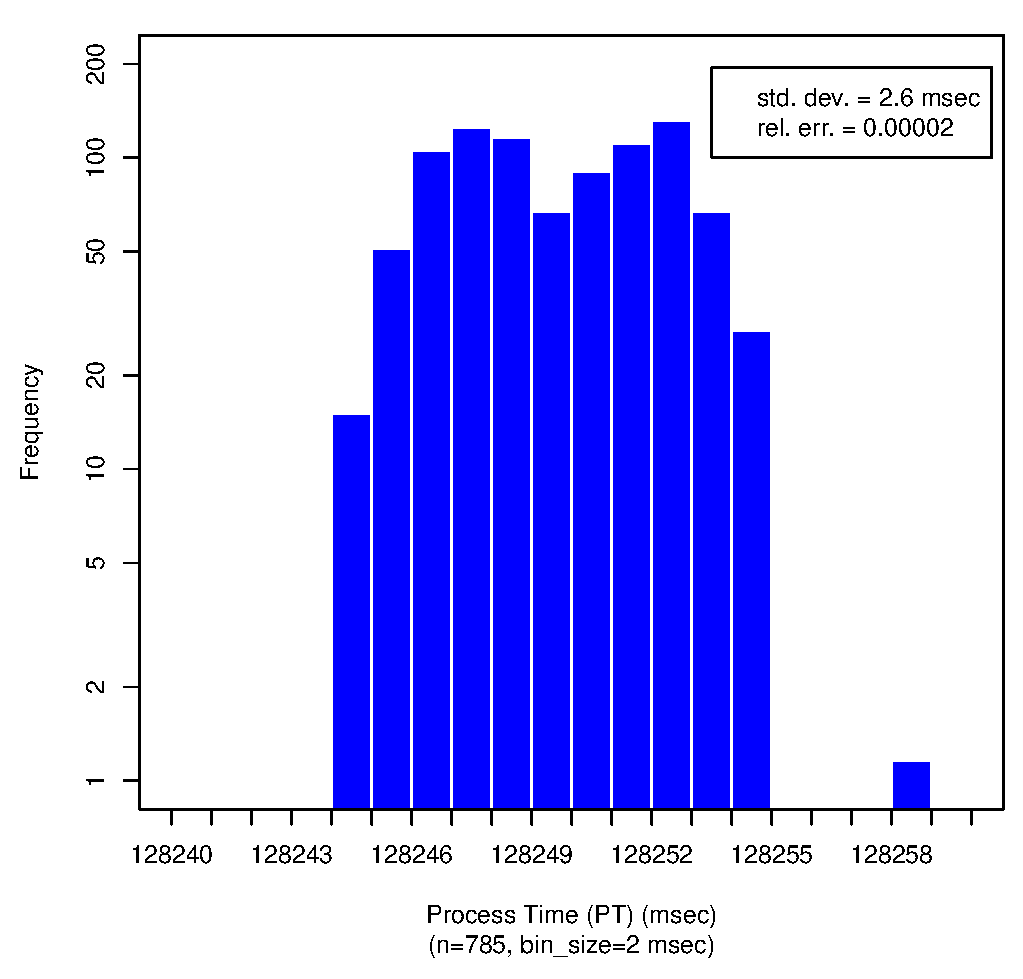
\includegraphics[width=0.31\textwidth]{128_sec_pt_new_hist.eps}
		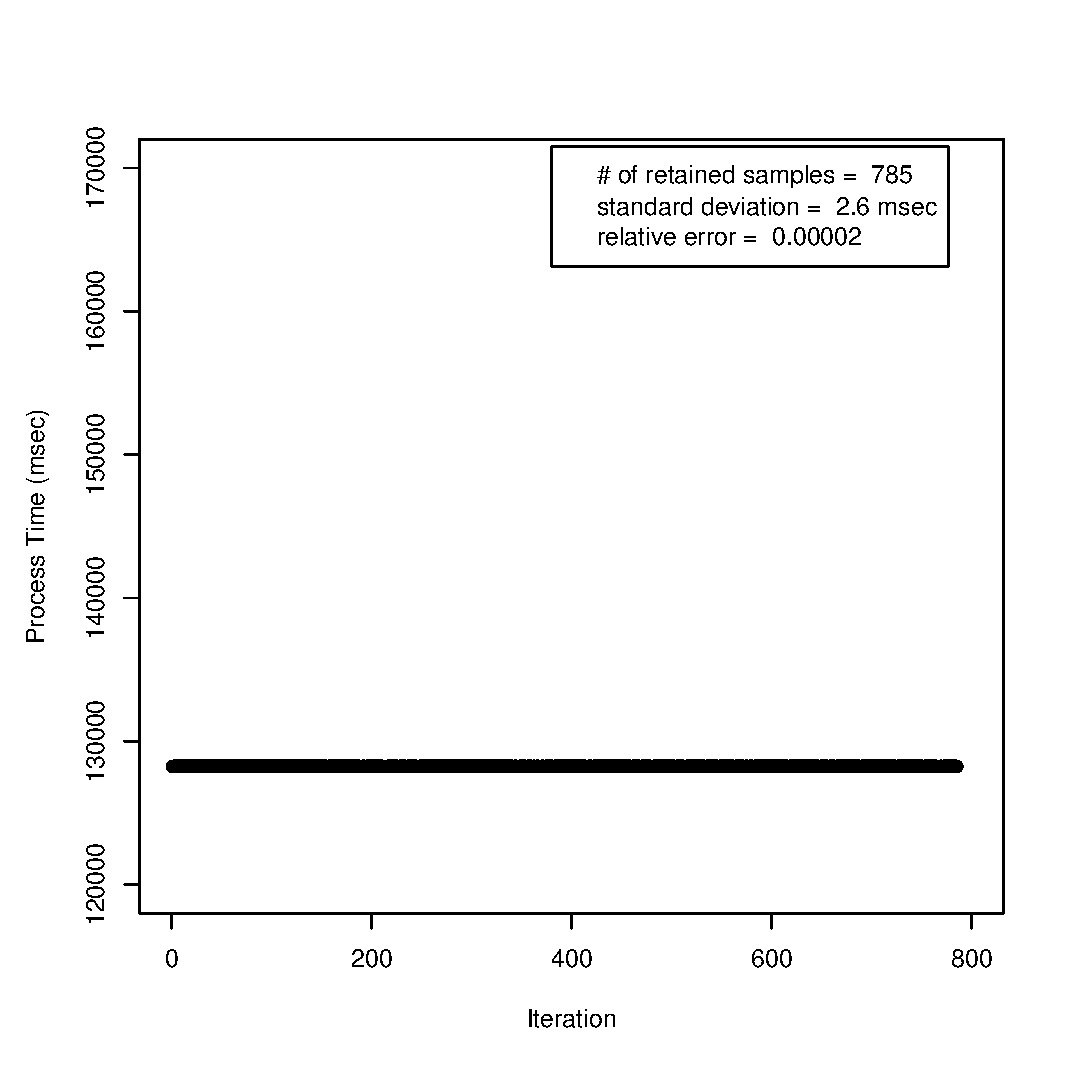
\includegraphics[width=0.224\textwidth]{128_sec_pt_new.eps}
		\label{fig:hist_after_pt}
	}
	\caption{An Example of Measurement Results on a \linebreak \hbox{Compute-bound} 
	Program-Under-Test~\label{fig:meas_comp}}
	\vspace{-.18in}
\end{figure} 

Commercial software tools measure execution time~\cite{VTune,TimeSys,WindView}. 
Since the tools' source code is not disclosed, there is no way of figuring out 
whether they can prevent such a daemon from timing. 

We previously developed a timing protocol called TTP (Tucson Timing Protocol)
for programs exhibiting I/O, in particular, query execution time in \hbox{DBMSes}~\cite{Currim}.
Our study identified a variety of Linux measures 
(e.g., user ticks, system ticks, IOWait ticks, etc.) 
relevant to timing a single query and then 
presented a structural causal model 
of explicating the variance of query time. 
Based on this model, we proposed the protocol for calculating the query time. 
Our scheme we propose in this manuscript 
is applicable to the TTP protocol, to further improve the query time calculation.

%\vspace{0.05in}
{\bf Contribution.} 
Our contributions are following.
\vspace{-0.12in}
\begin{itemize}

\item We show empirical evidence that 
measuring program time 
can be seriously affected by daemons.

\item We propose a novel timing protocol that
identifies infrequent, long-running daemons that impact the timing results for that program. 

\item We evaluate the performance of the protocol with rigorous experiments, 
starting from a simple program in pure-computation mode 
to a popular industrial benchmark suite.

\item The experimental results show a support for the effectiveness of our scheme\shorten{SEDONA: 
early eliminating dirty executions infected with such a daemon 
and eventually contributing to enhancing the overall measurement-quality}. 

\end{itemize}
\vspace{-0.05in}

\noindent
The rest of this letter is organized as follows. 
Section~\ref{sec:prop_appach} elaborates on the proposed scheme. 
In the following section, we evaluate the performance of 
the scheme using real workloads.

%\vspace\fill

\section{Proposed Scheme}
\label{sec:prop_appach}

In this section we propose a novel execution-time measurement scheme, 
called {\em SEDONA} (Selective Elimination through Detection of infrequent, lOng-ruNning dAemons). 
Our scheme catches and eliminates executions including daemon processes that are infrequent and 
long-running via a {\em cutoff} measure, and significantly improves measurement quality. 
The SEDONA protocol consists of a total of ten steps, as described in Fig.~\ref{alg:find}. 
%We first enumerate the steps to (a)~identify infrequent, 
%long-running daemons, using a single run of many executions of PUT128, 
%(b)~refine the list using a single run of many executions of PUT16384 (with a task length of 16K sec), 
%and then (c)~use the data from those two runs to determine the cutoff for 
%each \hbox{so-identified} daemon. 
%We can then apply these cutoffs to remove outliers from subsequent runs of any 
%arbitrary PUT and realistic workloads.
%\vspace{-0.22in}

\begin{figure}[h]
\begin{center}
\begin{algorithmic}
{\bf Algorithm} The SEDONA Timing Protocol: \\
\STATE Step 1. Set up the timing environment.
\STATE Step 2. Perform a single PUT run (specifically, PUT128) for many samples (specifically, 800).
\STATE Step 3. Consider each pair of elapsed time measurements to be a dual-PUT measurement 
and examine a scatter-plot to see if it it displays an $L$-shape.
\STATE Step 4. Zoom into the central cluster to ensure that it is symmetric (roughly circular).
\STATE Step 5. Compute the maximum and standard deviation of the process time 
for each daemon encountered within the central cluster samples.
\STATE Step 6. Identify for each sample in the $L$-shape infrequent, long-running daemon executions. 
\STATE Step 7. Determine potentially periodic daemons based on the $L$-executions 
and for each daemon compute the minimum process time from those executions identified. 
\STATE Step 8. Perform Steps 1--6 above for a single run 
consisting of a small number of executions (specifically, 40) of PUT16384.  
\STATE Step 9. Compute the cutoffs for each identified daemon. 
\STATE Step 10. Discard an execution including a daemon of which process time is greater than the respective cutoff time.
\end{algorithmic}
\end{center}
\caption{Summary of the SEDONA Timing Protocol\label{alg:find}}
\vspace{-0.25in}
\end{figure}
%

%We now elaborate the SEDONA scheme with an example, to explain and justify each step.
%\vspace{-0.8in}

%\subsection{A Running Example} 
%\vspace{-0.05in}
{\bf A Running Example.} 
As motivated by our prior work~\cite{Currim}, 
we configure a timing environment by i) stopping non-critical daemons, 
ii) activating the Network Timing Protocol daemon, and 
iii) switching off particular CPU features\cite{intel15,intelSpeed15} if any (Step 1). 
%(Our machine's specification will be given in Tab~\ref{tab:machine_config}).

We then run a program-under-test (called PUT) of 
Fig.~\ref{alg:put} with a task length of 128~sec, 
termed {\em PUT128}, 800 times (Step 2). 
(We render Fig.~\ref{fig:hist_before_et} using the 800 samples from this run.)
We use 128 seconds because that is long enough to perhaps experience an infrequent daemon. 
We run it 800 times to capture infrequent daemons that perhaps run every few hours or even 
once a day. 
Note that we collect all daemon processes as well as the PUT and their measures 
through the Netlink interface from the kernel before and after each 
timing.

Fig.~\ref{fig:reg_put128} plots all the 800 elapsed times of the run of PUT128.
%We see three rows in the plot: a solid row of many samples, perhaps
%six or more samples that are just above that solid row, and two
%samples that are way above the solid row. 
The plot clearly shows three rows; that is, 
the top and middle rows represent over a dozen of outliers far from 
the rest of the samples clustered in the bottom row. 
We'll now drill down into these outliers to 
show how to reliably eliminate the indirect influence of 
some ``infrequent, long-running daemons'' on the process time (PT) 
of the PUT.

To identify such daemons, we use a novel scatter plot: 
those of {\em pairs of successive samples}.\shorten{So samples 1 and 2 
form the first pair, samples 3 and 4 form the second pair.} 
Fig.~\ref{fig:raw_put128} presents such a scatter plot 
of 400 samples of a \hbox{dual-PUT256} constructed 
from a run of the 800 PUT128 samples (Step~3). 
There are two quite obvious outliers\shorten{, corresponding to sample \# 75 and \# 634,} with ETs of 163,913 msec (rightmost) and 161,785 msec (uppermost), respectively. 

\begin{figure}[t]
	\centering
	\subfigure[PUT128 with 800 Samples]{
		%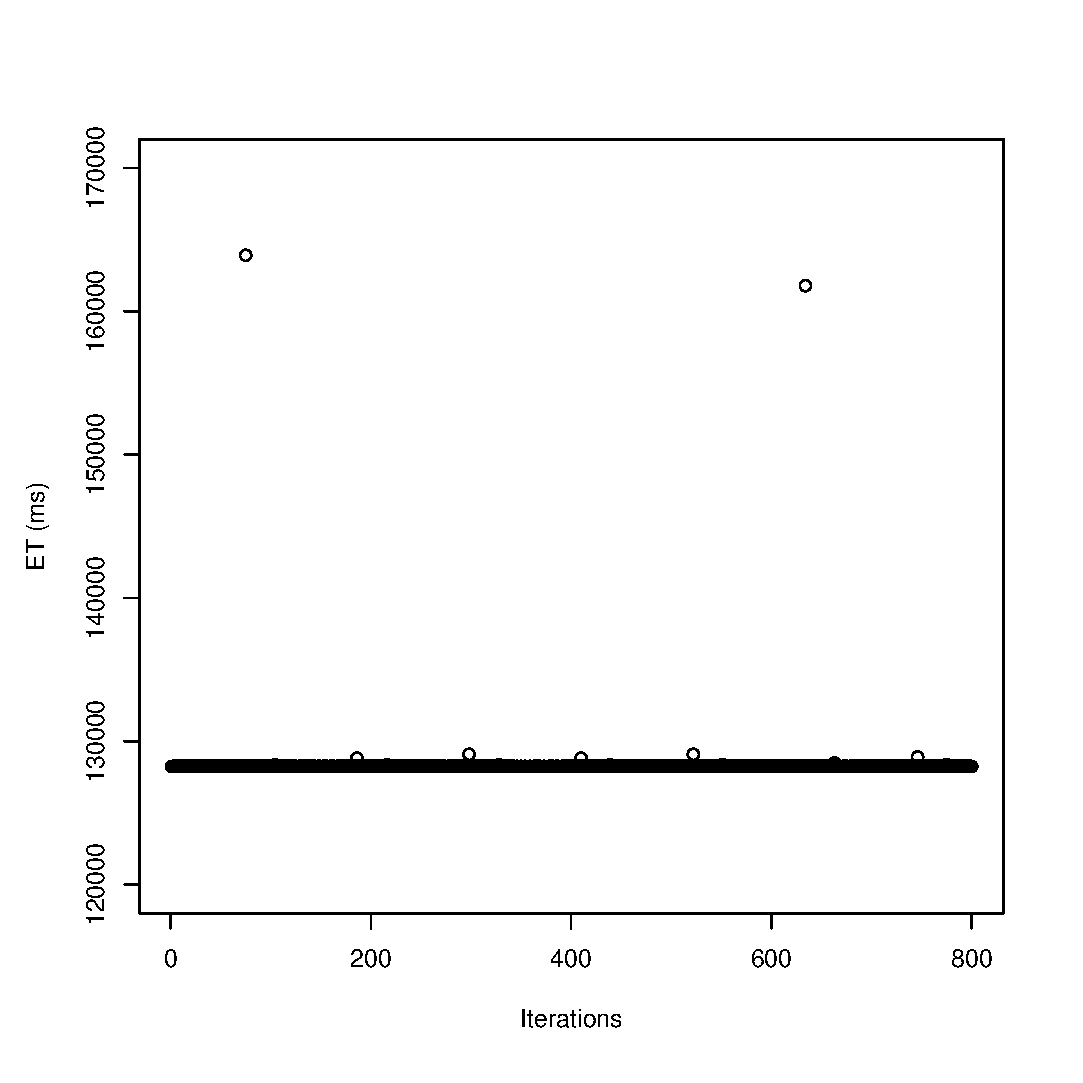
\includegraphics[width=0.223\textwidth]{put128_empv4.eps}
		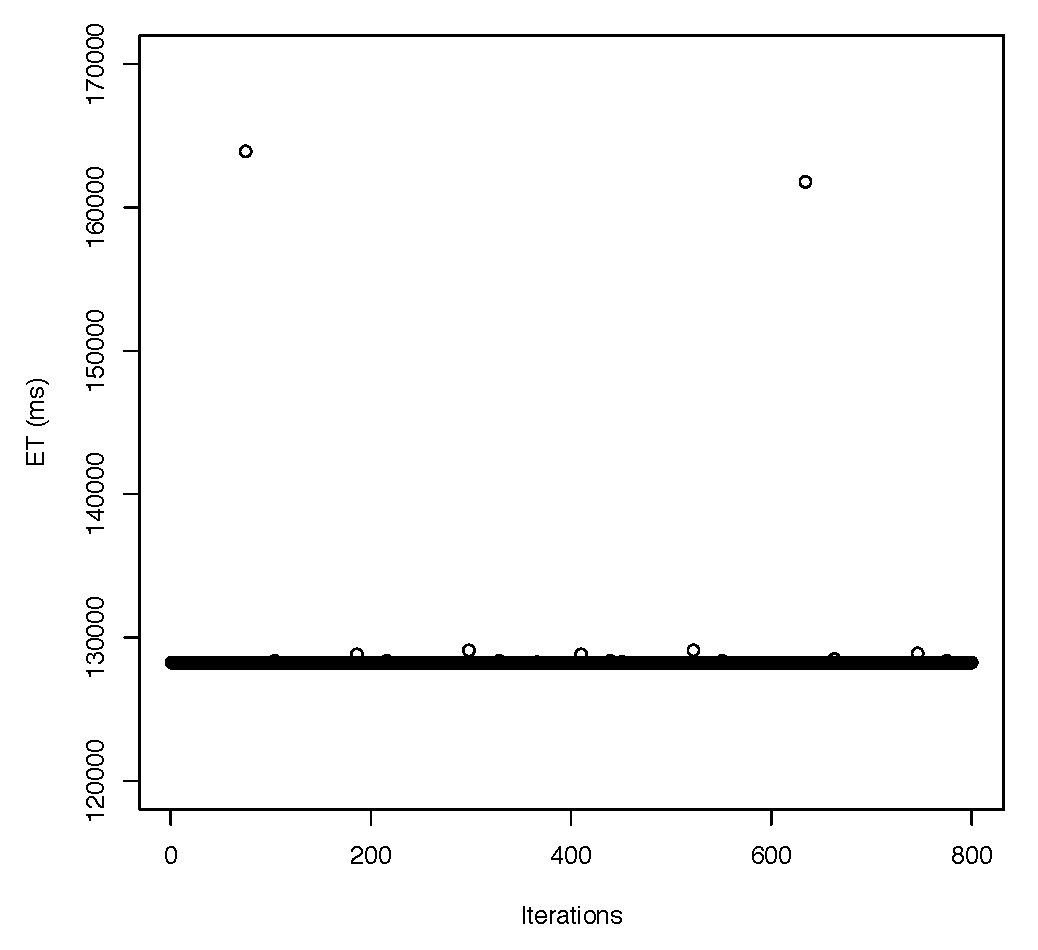
\includegraphics[width=0.224\textwidth]{put128_empv4_new.eps}
		\label{fig:reg_put128}
	}
	\subfigure[Dual-PUT256 Measurements]{
		%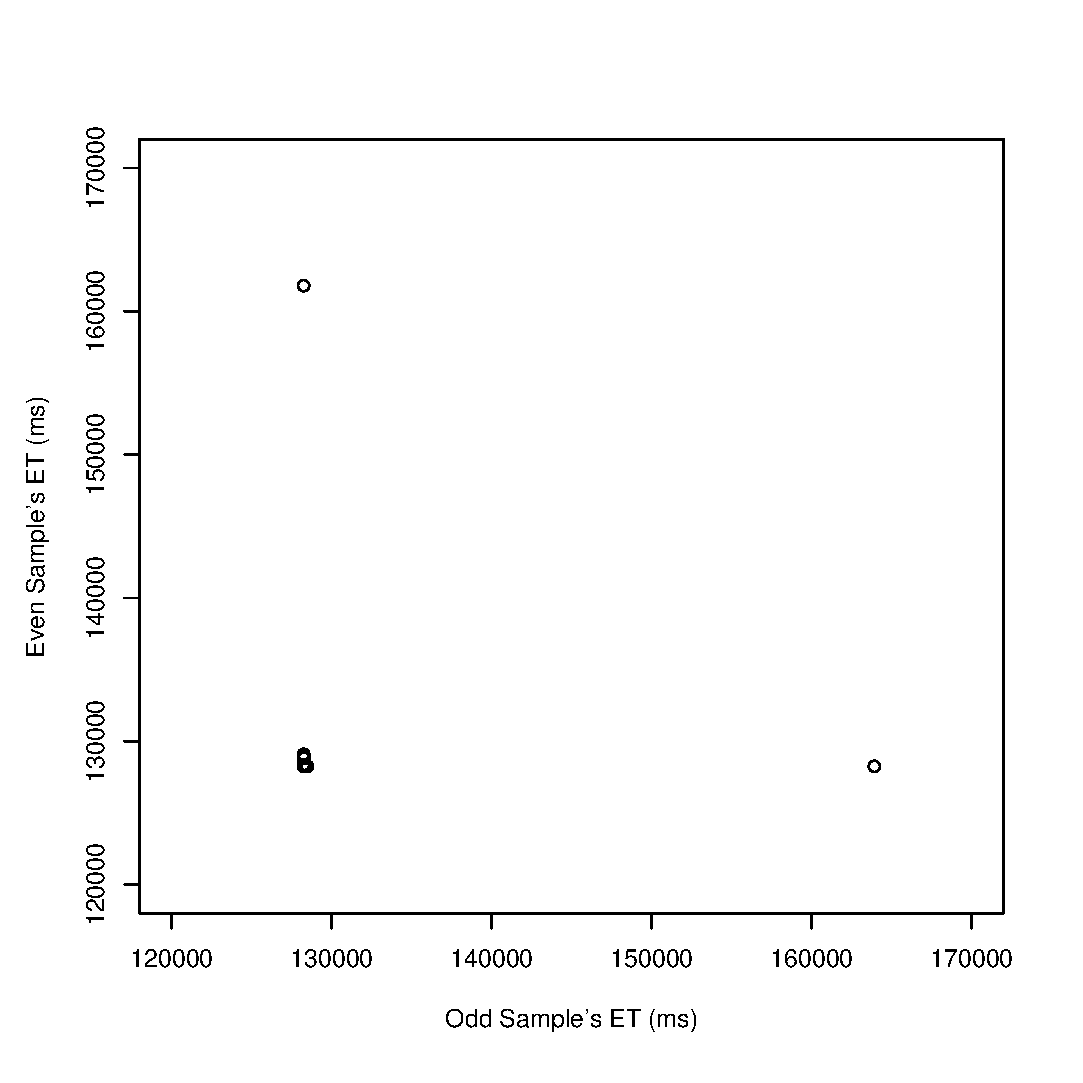
\includegraphics[width=0.223\textwidth]{dual_et_put256_empv4.eps}
		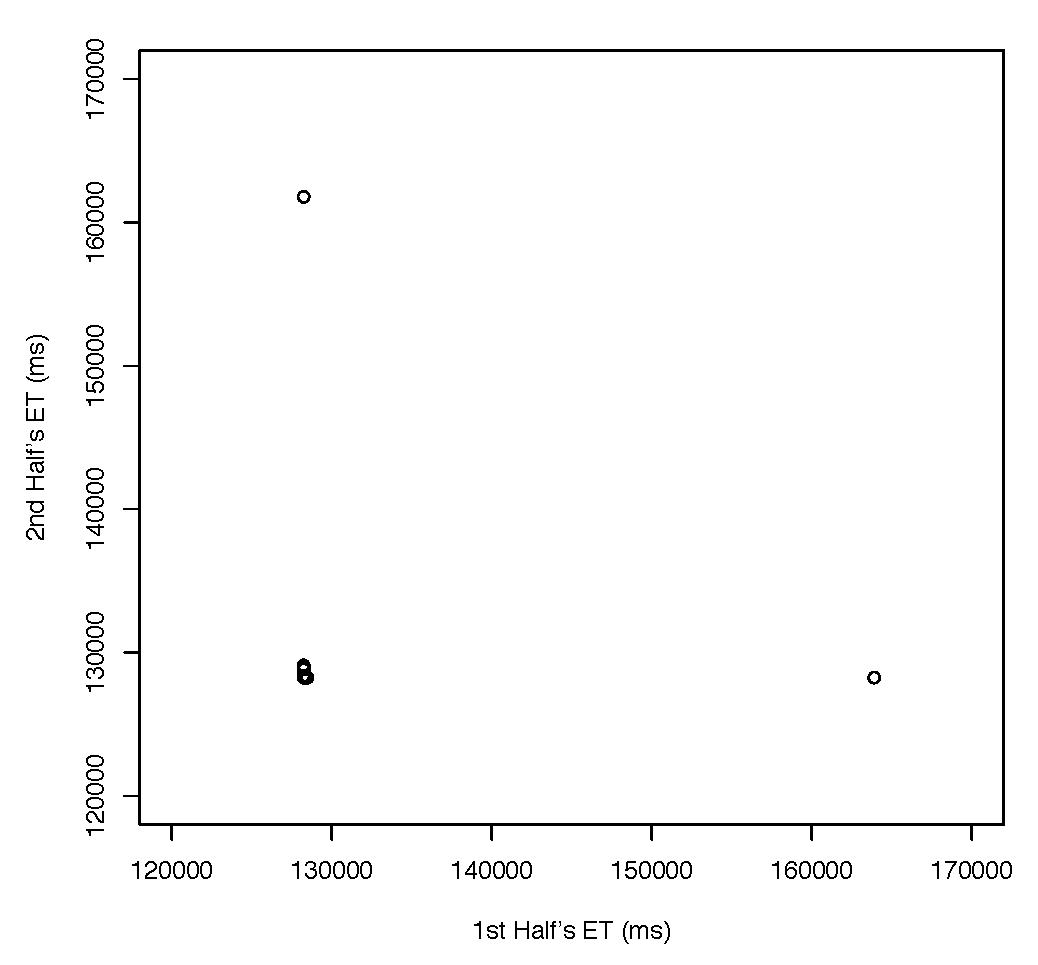
\includegraphics[width=0.224\textwidth]{dual_et_put256_empv4_new.eps}
		\label{fig:raw_put128}
	}
	\vspace{0.1in}    
	\subfigure[Zooming in on the $L$-shape]{
		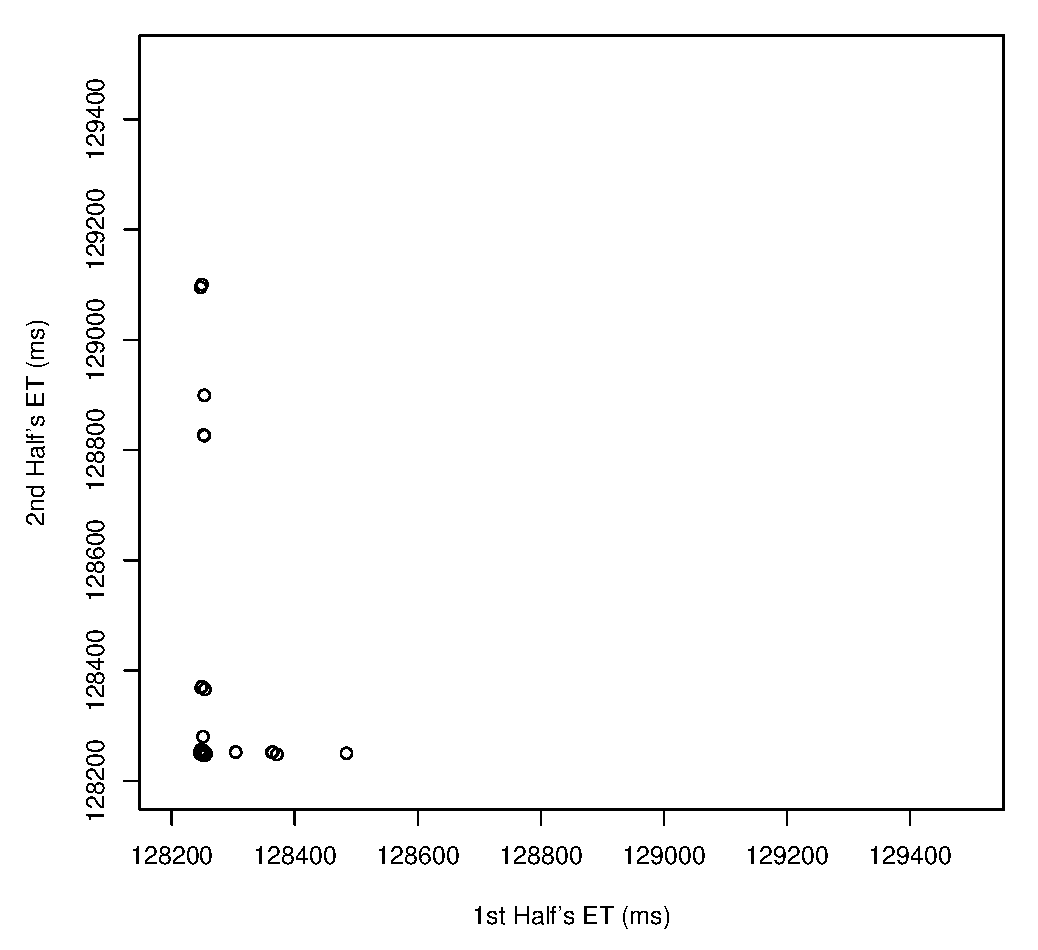
\includegraphics[width=0.224\textwidth]{zooming_in_dual_et_put256_empv4.eps}
		\label{fig:dual_put256_liters}
	}
%	\subfigure[Further Zooming in on the $L$-Shape]{
%		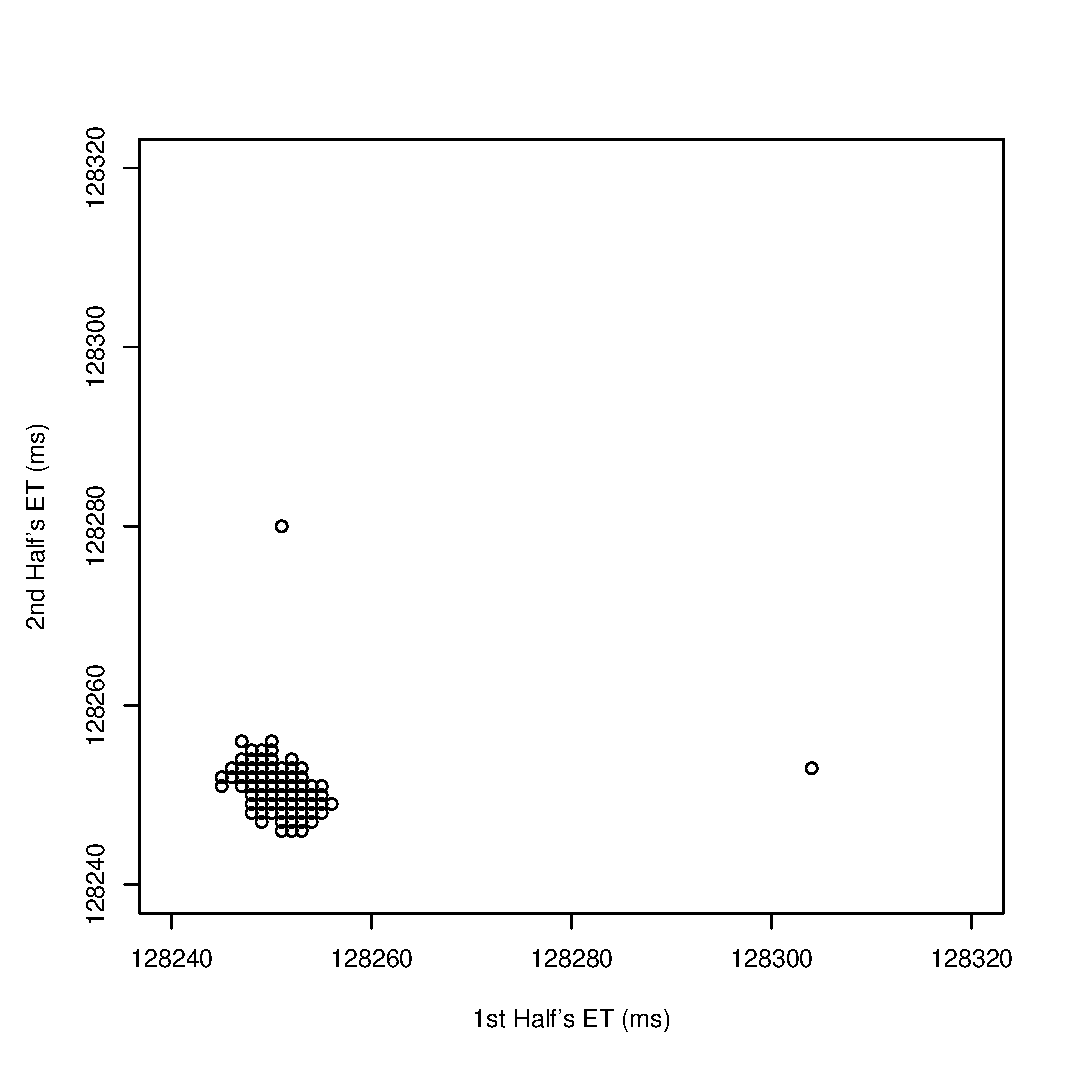
\includegraphics[scale=0.39]{further_zooming_in_dual_et_put256_empv4.eps}
%		\label{fig:fzoom_in_dual_et_put256}
%	}
	\subfigure[The Central Cluster]{
		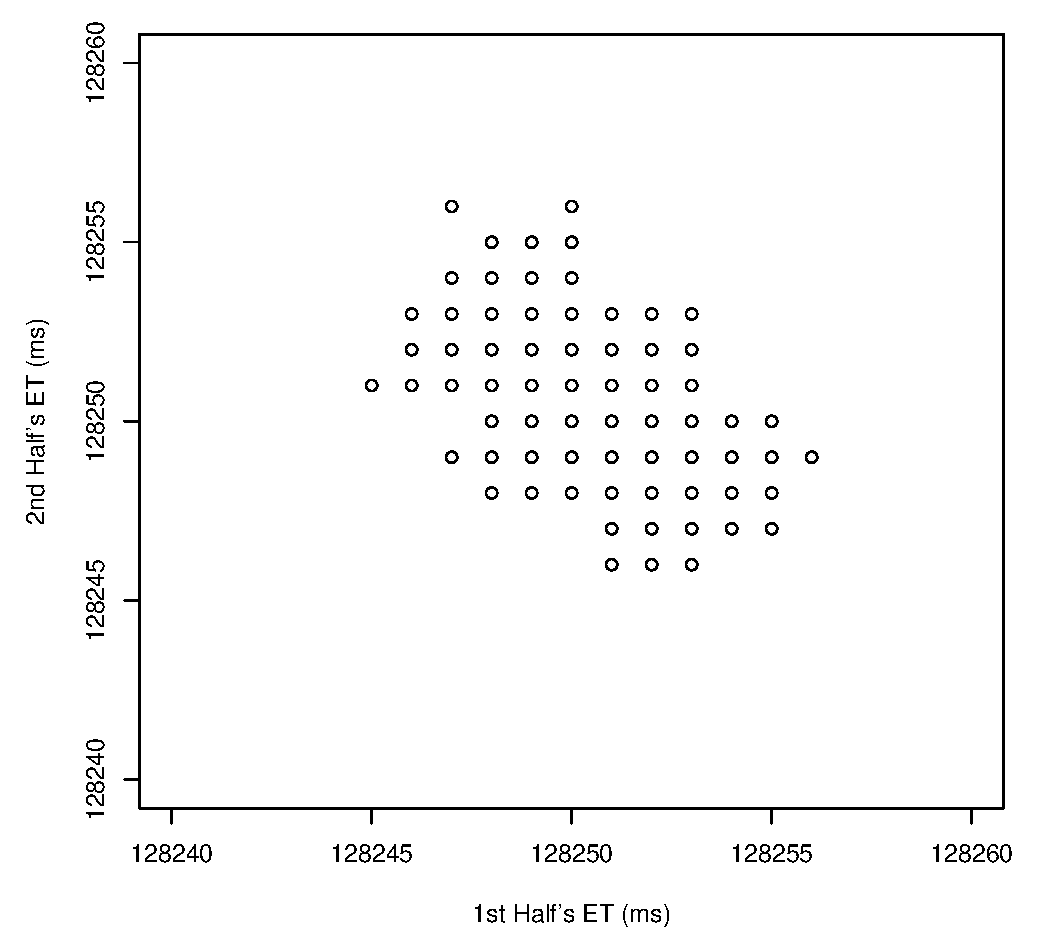
\includegraphics[width=0.224\textwidth]{dual_et_clump_put256_empv4.eps}
		\label{fig:dual_et_put256_cluster}
        }
    \caption{Successive Scatter plots of a PUT128 with 800 samples 
    (equivalent to a Dual-PUT256 with 400 samples) in Steps~2---4~\label{fig:put128_plot}} 
    \vspace{-0.16in}     
\end{figure} 

We informally term this phenomenon of a scatter plot of a dual-PUT run an
``$L$-shape,'' and attribute it to the
presence of infrequent long-running daemons.\shorten{Again, samples containing such
daemons (termed the $L$-samples) will appear
along the left y-axis or along the bottom x-axis, but will not occur in the
top right of the scatter plot of the dual-PUT.}

Figure~\ref{fig:dual_put256_liters} zooms into the lower left region,
focusing on the
tight cluster of samples.  Interestingly, this plot continues to exhibit an
$L$-shape, with perhaps a dozen or more $L$-samples in the left and bottom arms of
the ``$L$,'' and again no samples in the upper right portion of the
scatter plot.

We continue zooming until we get to Figure~\ref{fig:dual_et_put256_cluster},
which shows a central cluster (Step 4). 
We confirm the symmetry of the ET measurements in the central cluster: there
is no $L$-shape, and thus no $L$-samples, and thus no obvious infrequent
long-running daemons.\shorten{(We emphasize that these samples may have lots of
frequent daemons, as well as infrequent, {\em short-running} daemons.) There
were 384 dual-PUT256 samples in this central cluster, implying that 16 of
the PUT128 samples were $L$-samples and the 785 remaining of the original 800 PUT128
samples had no infrequent, long-running daemons, which motivates that term.}

We then perform Step~5, which computes 
the maximum process time and standard deviation 
of PT (process time, note the switch in emphasis from elapsed time 
to process time) of the daemon processes 
(e.g. {\tt cifsd}, {\tt flush-9:0}, {\tt jbd2/md0-8}, 
{\tt kblockd/0}, {\tt khugepaged}, {\tt md0\_raid1}, and {\tt ntpd})
observed in the central cluster samples in Fig.~\ref{fig:dual_et_put256_cluster}. 
\shorten{In the running example the maximum PT of those daemons was under 4 msec, 
and their standard deviation was just about 1 msec.}

In Step~6 we identify, for each daemon in the \hbox{$L$-samples}, 
those that are actual long-running daemon
executions.  We define such executions as those whose PT 
is over two standard deviations above the maximum PT for
that daemon in the central cluster samples. 
In the running example  {\tt flush-9:0}, 
{\tt jbd2/md0-8}, and {\tt md0\_raid1} 
are determined as infrequent, long-running.
We also identify ``extra'' infrequent daemons: those
found only in the $L$-samples but not in the central cluster. 
The running example reveals the following extra daemons: 
{\tt bash}, {\tt grep}, {\tt rhn\_check}, {\tt rhnsd}, {\tt rhsmcertd}, 
{\tt rhsmcertd-worke}, and {\tt sshd}.

For each of the infrequent daemons 
we use a heuristic to determine the daemon's periodicity: 
the daemon must occur regularly in a sequence of samples.
For instance, the {\tt rhn\_check} daemon appears 
roughly every 112 samples (which corresponds to very close to every four 
hours). Four others ({\tt flush-9:0}, {\tt jbd2/md0-8}, 
{\tt md0\_raid1}, and {\tt rhn\_check}) all occur together 
(in those two outliers in Fig.~\ref{fig:raw_put128}) and 
  have a periodicity of about every 559 samples
  (5x longer, or just about 20 hours). 
%  It is important only which samples a given daemon shows up 
%  in; we don't care in this heuristic whether daemons are co-occurring.

Next, we can compute for each so-identified infrequent, long-running daemon its
minimum time in the \hbox{$L$-samples} (Step 7). 
This computation provides a rough, initial distinction of a ``long-running''
daemon, namely, the valley between the maximum PT from the central cluster 
and the minimum PT from the $L$-samples, to differentiate ``short-running'' 
from ``\hbox{long-running}'' executions of the daemon. 
For those daemons (i.e. {\tt grep}) never appearing in the central cluster,
this initial analysis concludes only that they are infrequent.

In Step 8 we repeat Steps 1--6, but instead with the much-longer running
PUT16384 (4.5 hours per \hbox{sample} versus 2 minutes), to see 
if any of our identified \hbox{infrequent} daemons are actually frequent 
at that much longer PUT execution time. 
We find some frequent daemon processes appearing in both of the 
clusters of the dual-PUT256 and dual-PUT32768: 
{\tt flush-9.0}, {\tt jbd2/md0-8}, {\tt kblock/0}, {\tt md0\_raid1}, 
and {\tt ntpd}. That said, the central cluster also contains other
  processes not seen in the dual-PUT256 central cluster: 
  {\tt grep}, {\tt rhn\_check}, {\tt rhnsd}, {\tt rhsmcertd}, 
  {\tt rhsmcertd-worke}, and {\tt sshd}. 
  But these daemons were categorized in the \hbox{dual-PUT256} analysis as {\em
  infrequent}, several having \hbox{periodicities} estimated at four or twenty hours.
When the PUT had a ``short'' 
program time (in this case, two minutes), daemons with a periodicity of
hours are \hbox{infrequent}. But with a PUT with a ``long'' program time (in this
case, 4.5 hours), some of those daemons are now frequent, and appear in the 
central cluster.

In Step~9 we compute 
the cutoff for each of those infrequent, long-running daemons so
identified, based on the PUT128 and the 
PUT16384 as collected in Tab.~\ref{tab:final_infrequent_cutoff}. 
Here is how to compute the cutoff. For the cutoff of such a daemon with PUT128, 
we take the \hbox{midpoint} between the maximum of that daemon's PTs in the 
central cluster (or 0, if absent) and the \hbox{minimum} of those in the $L$-samples. 
For the cutoff of such a daemon with PUT16384, we do the same. 
We then compute a ``task time'' as 5\% of the inferred periodicity. 
This 5\% ensures that such infrequent daemons will impact 
only a small percentage of the shorter PUTs, while presumably being 
associated with much larger cutoffs for the very long PUTs. 
We also include daemons that (a)~were identified as infrequent and 
\hbox{long-running} from PUT128 and (b)~were not identified as so in the PUT16384 
\hbox{$L$-samples}, but may have in the \hbox{dual-PUT32768} central cluster. 
We then take the {\em maximum} of the two cutoffs for the final cutoff PT 
(the last column of Tab.~\ref{tab:final_infrequent_cutoff}). 

\begin{table}[h]
\centering
{\scriptsize
\begin{tabular}{|p{1.2cm}|c|c|p{1cm}|p{1.45cm}|} \hline
{\tiny Process}  & {\tiny Cutoff PT} & {\tiny Cutoff PT} & {\tiny Task}  & {\tiny{\bf Final }} \\
{\tiny Name} & {\tiny on PUT128}  & {\tiny on PUT16K} & {\tiny Time} & {\tiny {\bf Cutoff PT}} \\\hline
%{\tiny Process}  & {\tiny Cutoff PT} & {\tiny Cutoff PT} & {\tiny Task}  & {\tiny{\bf Final }} \\
% Name & on PUT128  & on PUT16K & Time & {\bf Cutoff PT} \\\hline
{\tt bash} & 1 msec & --- & --- & {\bf 1 msec} \\ \hline
{\tt flush-9:0} & 64 msec & --- & $< 1$ hour & {\bf 64 msec} \\
                & ---     & 48 msec & $\geq 1$ hour & {\bf 48 msec} \\ \hline
{\tt grep }     & 1 msec & 12 msec & --- & {\bf 12 msec}\\ \hline
{\tt jbd2/md0-8} & 4 msec & --- & $< 1$ hour & {\bf 4 msec} \\
                & ---     & 11 msec & $\geq 1$ hour & {\bf 11 msec} \\ \hline
{\tt md0\_raid1} & 35 msec & ---     & $< 1$ hour  & {\bf 35 msec}\\
                 & ---     & 51 msec & $\geq 1$ hour & {\bf 51 msec} \\ \hline
{\tt rhn\_check}  & 281 msec & --- & $< 12$ min & {\bf 281 msec} \\
                 &  --- & 12,828 msec & $\geq 12$ min & {\bf 12,828 msec}\\ \hline
{\tt rhnsd} & 2 msec & --- & $< 12$ min & {\bf 2 msec} \\
            & ---    & 12 msec &$\geq 12$ min & {\bf 12 msec} \\ \hline
{\tt rhsmcertd}  & 1 msec & 1 msec & --- & {\bf 1 msec} \\  \hline
{\tt rhsmcertd}  & 57 msec & --- & $< 12$ min & {\bf 57 msec} \\
{\tt -worke}           &  --- & 119 msec  & $\geq 12$ min & {\bf 119 msec}\\ \hline
{\tt sshd} & 2 msec & 23 msec & --- & {\bf 23 msec}\\ \hline
\end{tabular}
}
\caption{Collected Infrequent, Long-running Daemons and Their Final Cutoff
  Process Time \hbox{(Step~9)}\label{tab:final_infrequent_cutoff}}
  \vspace{-0.4in}
\end{table}

Based on Tab.~\ref{tab:final_infrequent_cutoff}, 
we discard any \hbox{sample} \hbox{containing} an infrequent, long-running daemon execution
over the corresponding cutoff. We thus end up dropping just fifteen of the 800
PUT128 samples and only two of the forty PUT16384 samples. 
As a result, the \hbox{overall} \hbox{measurement} quality---the standard deviation and \hbox{relative} error 
---for PUT128 was improved 
by three orders of magnitude (as shown in Fig.~\ref{fig:meas_comp}) 
and by about two \hbox{orders} of magnitude for PUT16384.
%(5661.7 vs. 229.8) 0.0003448491 vs. 8.4$\times$10$^{-6}$
%(40.4 vs. 26.7) 2.463122e-06 vs. 1.626005e-06

\vspace\fill

\section{Evaluation}
\label{sec:eval}
\vspace{-0.07in}
We now evaluate the \hbox{performance} of the SEDONA \hbox{protocol}.
Our experiments were conducted on a \hbox{machine}
described in Table~\ref{tab:machine_config}. 
\begin{table}[h]
\vspace{-0.2in}
\begin{center}
{\scriptsize
\begin{tabular}{|l|p{7cm}|}\hline
OS & Red Hat Ent. Linux (RHEL) 6.4 with a kernel of 2.6.32 \\ \hline
CPU & Intel Core i7-870 Lynnfield 2.93GHz quad-core \hbox{processor}\shorten{ on a LGA 1156 95W motherboard}\\ \hline
RAM & 4GB of DDR3 1333 dual-channel memory\\ \hline
HDD & Western Digital Caviar Black 1TB 7200rpm SATA Drive\\ \hline
\end{tabular}
}
\end{center}
\caption{Machine Configurations\label{tab:machine_config}}
\vspace{-0.3in}
\end{table}

We evaluated the performance of SEDONA \hbox{using} SPEC CPU2006 
benchmarks~\cite{specCpu2006}, providing \hbox{various} compute-bound real applications. 
%Thus, employing the SPEC benchmarks as real-world workloads 
%was a reasonable choice for the evaluation. 
The results are \hbox{provided} in Table~\ref{tab:spec_real}. 
Note that in the table the results for {\tt 481} and {\tt 483} \hbox{benchmarks} 
are omitted because of some runtime error and incurred I/O, respectively.

{\color{blue}
We compared the performance of ORG and \hbox{SEDONA} on 
real programs such as insertion sort, termed SORT and 
matrix multiplication (in column major), termed MM. 
SEDONA overwhelmed ORG, as can be seen in Fig.~\ref{fig:synprog_test}. 
As workload size increased, 
the performance gap between SEDONA and ORG got increasingly widened, reaching up to by 6x.

\begin{figure}[htp!]
	\centering
	\subfigure[SORT - Standard Deviation]{
		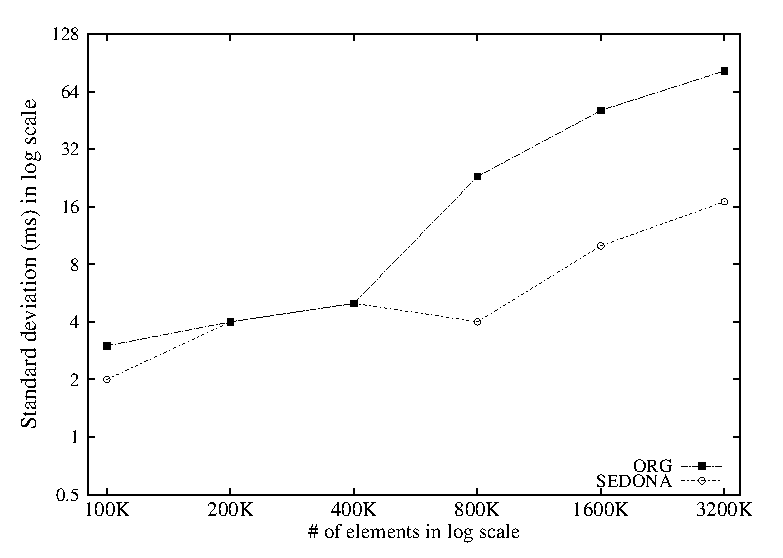
\includegraphics[scale=0.31]{sort_std.eps}
		\label{fig:sort_std}
	}
	\subfigure[SORT - Relative Error]{
		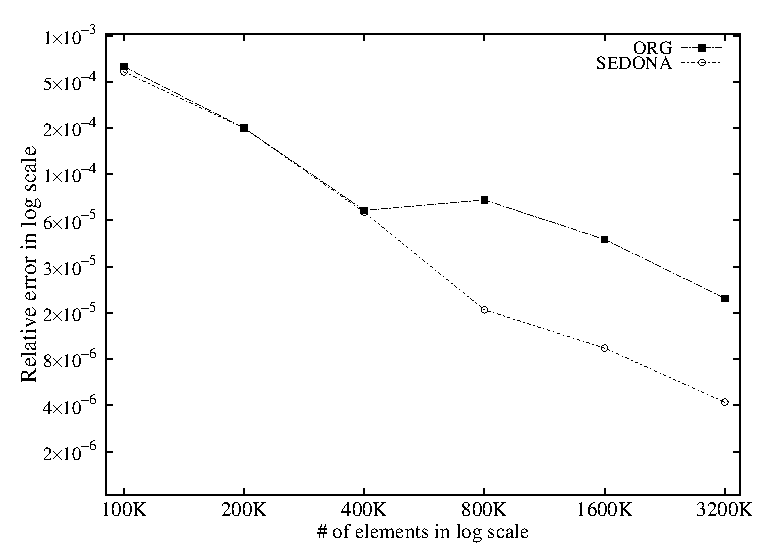
\includegraphics[scale=0.31]{sort_re.eps}
		\label{fig:sort_re}
	}
	\subfigure[MM - Standard Deviation]{
		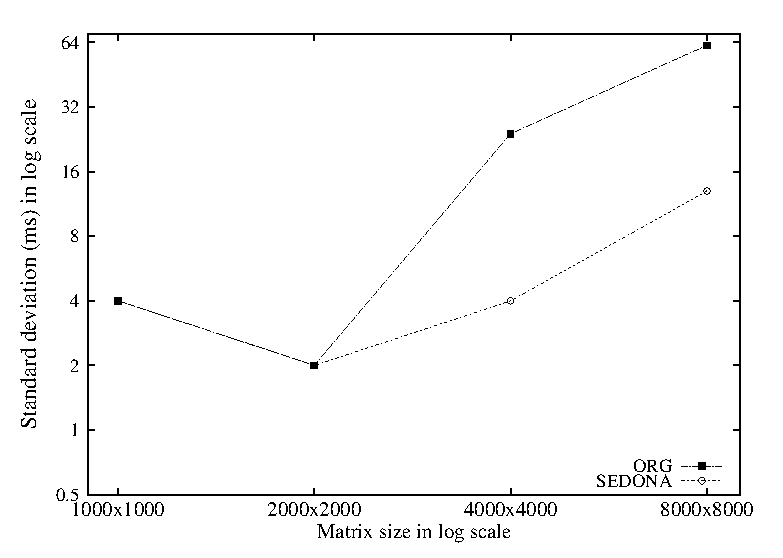
\includegraphics[scale=0.31]{matc_std.eps}
		\label{fig:matc_std}
	}
	\subfigure[MM - Relative Error]{
		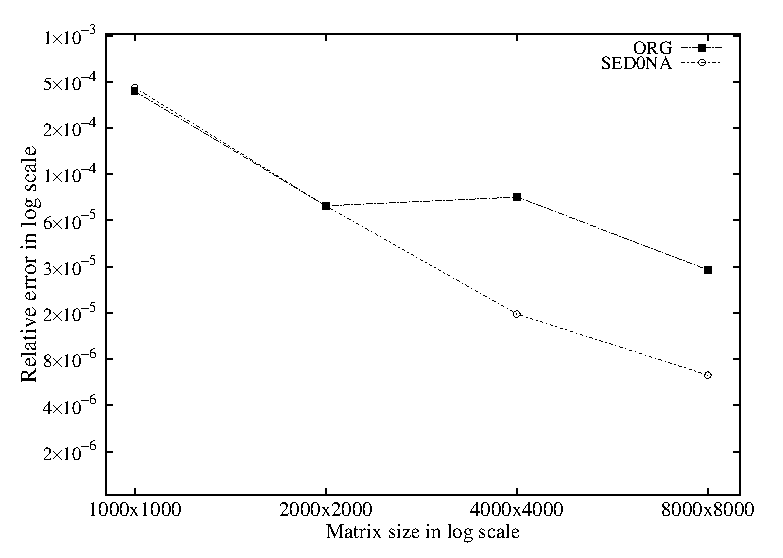
\includegraphics[scale=0.31]{matc_re.eps}
		\label{fig:matc_re}
	}
	\vspace{-.1in}
	\caption{Performance Comparison on Real-world Programs~\label{fig:synprog_test}}
\vspace{-.2in}
\end{figure}
}

Table~\ref{tab:spec_real} shows that
the SEDONA protocol (which uses PT) significantly outperformed the original 
measurement technique (using ET), termed ORG, 
on the standard deviation and relative error across the different SPEC benchmarks. 
None of the benchmarks revealed a bigger standard deviation from the SEDONA protocol as compared to that of ORG. 
%All of the benchmarks revealed a smaller standard deviation on our scheme than that of the ORG. 
Our protocol quite effectively filtered out infrequent daemon executions 
in these real-world workloads. 
Furthermore, the relative error of SEDONA was 
lower than that of ORG for all the benchmarks. 
For instance, about a 10x \hbox{margin} between the two was yielded for 
{\tt 434.zeusmp}.

SEDONA also scaled well for the SPEC workloads, 
with regard to growth of relative error as the execution time lengthened.
For the short benchmarks 
(e.g., {\tt 400}, {\tt 403}, {\tt 410}, 
{\tt 434}, {\tt 445}, and {\tt 999}: those taking \hbox{under} 100 sec), 
our scheme outperformed the ORG by about 3.5x, on average. 
The SEDONA protocol continued its dominance against the conventional technique 
for the medium-length benchmarks (e.g., {\tt 447}, {\tt 456}, {\tt 470}, and {\tt 473}).
For the long-running benchmarks (e.g., {\tt 436} and {\tt 454}, both$>$ 1,000 sec), 
the relative error of \hbox{SEDONA} was slightly lower than that of ORG.

%Lastly, the average standard deviation and relative error of the SEDONA 
%among all the benchmarks were smaller that those of the ORG, 
%as indicated by the last two rows. 
%Lastly, the SEDONA outperformed the ORG by a slight margin \hbox{regarding} 
%the plain (un-weighted) and weighted averages of 
%the standard deviation and relative error among all the benchmarks, 
%as indicated by the last two rows.
%\shorten{In particular, the SEDONA outperformed the ORG regarding 
%the weighted average by normalization by a slight margin 
%in spite of seemingly being equal because of the rounding up to one significant digit.}
 
%Lastly, we still observed a substantial standard deviation (and relative error) for 
%some benchmarks (e.g., {\tt 436} and {\tt 462}).
%The high variance seemed mainly attributed to the activities
%of the {\tt kslowd000} and {\tt kslowd001} daemon processes, 
%as also identified in the real-world programs. 
%These two were not observed during our cutoff study. 
%The daemons cannot be switched off, as they involve kernel threads. 
%More investigation is needed to hopefully better remove 
%daemon executions interfering with timing a program.

To summarize, our proposed SEDONA protocol can achieve {\em better} accuracy,
precision, and scalability in measuring the execution time of real \hbox{compute-bound} benchmarks 
than the conventional timing method.

\vspace{-0.1in}
\begin{table}[h]
\centering
{
\scriptsize
%\tiny
%\begin{tabular}{|r|r|r|r|r|r|r|} \hline
% 		  & \multicolumn{2}{r|}{Execution Time (ms)} & \multicolumn{2}{r}{Standard} & \multicolumn{2}{|r|}{\multirow{2}{*}{Relative Error}}\\ \cline{2-3}
%SPEC  & {ORG}  & {SEDONA} 	& \multicolumn{2}{r}{Deviation (ms)} 	 					& \multicolumn{2}{|r|}{}\\ \cline{4-7}	
%		 & {(in ET)} &  {(in PT)} & {ORG} & {SEDONA} & {ORG} & {SEDONA}\\ \hline

%\begin{tabular}{|p{0.6cm}|p{1cm}|p{1cm}|p{0.5cm}|p{1cm}|p{0.8cm}|p{1cm}|} \hline
%		  & \multicolumn{2}{p{2.3cm}|}{Execution Time (ms)} & \multicolumn{2}{p{1.6cm}}{Standard}  & \multicolumn{2}{|l|}{\multirow{2}{*}{Relative Error}}\\ \cline{2-3}
%SPEC  & {ORG}  & {SEDONA} & \multicolumn{2}{p{1.6cm}}{Deviation(ms)} & \multicolumn{2}{|c|}{}\\ \cline{4-7}	
%		 & {(in ET)} &  {(in PT)} & {ORG} & {SEDONA} & {ORG} & {SEDONA}\\ \hline

\begin{tabular}{|p{0.18cm}|R{1.14cm}|R{1.14cm}|R{0.64cm}|R{1cm}|R{0.97cm}|R{0.97cm}|} \hline
 		  & \multicolumn{2}{c|}{{\tiny Execution Time (ms)}} & \multicolumn{2}{c|}{{\tiny Standard}}   & \multicolumn{2}{c|}{\multirow{2}{*}{{\tiny Relative Error}}}\\ \cline{2-3}
 & \multicolumn{1}{c|}{{\tiny{ORG}}}  & \multicolumn{1}{c|}{{\tiny{SEDONA}}} & \multicolumn{2}{c|}{{\tiny Deviation (ms)}}  & \multicolumn{2}{c|}{}\\ \cline{4-7}	
 & \multicolumn{1}{c|}{{\tiny{(in ET)}}} & \multicolumn{1}{c|}{{\tiny{(in PT)}}} & {\tiny{ORG}} & {\tiny{SEDONA}} & \multicolumn{1}{c|}{{\tiny{ORG}}}& \multicolumn{1}{c|}{{\tiny{SEDONA}}}\\ \hline
{{\tt 400}} & 454 & 445 & {3} & {2} & {6$\times$10$^{-3}$} & {3$\times$10$^{-3}$}\\
{{\tt 401}} & 536,639 & 528,517 & {1,185} & {1,161} & {2$\times$10$^{-3}$} & {2$\times$10$^{-3}$}\\
{{\tt 403}} & 26,109	& 25,695 & {138} & {96} & {5$\times$10$^{-3}$} & {4$\times$10$^{-3}$}\\
{{\tt 410}} & 7,938 & 7,801 & {46} & {19} & {6$\times$10$^{-3}$} & {2$\times$10$^{-3}$}\\
{{\tt 416}} & 1,015,342 & 999,846 & {965} & {876} & {1$\times$10$^{-3}$} & {9$\times$10$^{-4}$}\\%% V
{{\tt 429}} & 235,811 & 232,209 & {623} & {600} & {3$\times$10$^{-3}$} & {3$\times$10$^{-3}$}\\
{{\tt 433}} & 480,586 & 473,256  & {743} & {725} & {2$\times$10$^{-3}$} & {2$\times$10$^{-3}$}\\ %% V
{{\tt 434}} & 16,495  & 16,242  & {75} & {7} & {5$\times$10$^{-3}$} & {5$\times$10$^{-4}$}\\
{{\tt 435}} & 990,575 & 975,445  & {947} & {900} & {1$\times$10$^{-3}$} & {9$\times$10$^{-4}$}\\
{{\tt 436}} & 1,160,742 & 1,143,078   & {3,914} & {3,843} & {3$\times$10$^{-3}$} & {3$\times$10$^{-3}$}\\
{{\tt 437}} & 581,635 & 572,775 & {1,492} & {1,475}  & {3$\times$10$^{-3}$} & {3$\times$10$^{-3}$}\\
{{\tt 444}} & 591,201 & 582,229 & {294} & {281}  & {5$\times$10$^{-4}$} & {5$\times$10$^{-4}$}\\
{{\tt 445}} & 84,435  & 83,164  & {91} & {28}  & {1$\times$10$^{-3}$} & {3$\times$10$^{-4}$}\\
{{\tt 447}} & 521,846 & 513,493  & {150} & {108}  & {3$\times$10$^{-4}$} & {2$\times$10$^{-4}$}\\
{{\tt 450}} & 341,030 & 335,848  & {99} & {91}  & {3$\times$10$^{-4}$} & {2$\times$10$^{-4}$}\\
{{\tt 453}} & 258,797 & 254,496  & {623} & {582}  & {2$\times$10$^{-3}$} & {2$\times$10$^{-3}$}\\
{{\tt 454}} & 1,721,804 & 1,695,613  & {678} & {627}  & {4$\times$10$^{-4}$} & {4$\times$10$^{-4}$}\\
{{\tt 456}} & 410,533 & 404,328  & {85} & {50}  & {2$\times$10$^{-4}$} & {1$\times$10$^{-4}$}\\
{{\tt 458}} & 589,541 & 580,591  & {542} & {513} &  {9$\times$10$^{-4}$} & {9$\times$10$^{-4}$}\\
{{\tt 459}} & 798,917 & 786,726  & {2,143} & {2,132}  & {3$\times$10$^{-3}$} & {3$\times$10$^{-3}$}\\
{{\tt 462}} & 595,188 & 586,120  & {3,326} & {3,274}  & {6$\times$10$^{-3}$} & {6$\times$10$^{-3}$}\\
{{\tt 464}} & 649,838 & 639,939  & {601} & {563}  & {9$\times$10$^{-4}$} & {9$\times$10$^{-4}$}\\
{{\tt 465}} & 895,754 & 882,106  & {883} & {797}  & {1$\times$10$^{-3}$} & {1$\times$10$^{-3}$}\\
{{\tt 470}}	& 349,830 & 344,510 & {143} & {94} & {4$\times$10$^{-4}$} & {3$\times$10$^{-4}$}\\
{{\tt 471}} & 367,589 & 361,959  & {2,114} & {2,072} & {6$\times$10$^{-4}$} & {6$\times$10$^{-4}$}\\
{{\tt 473}} & 362,587 & 357,090  & {359} & {317} &  {1$\times$10$^{-3}$} & {9$\times$10$^{-4}$}\\
%{{\tt 481}} & \multicolumn{4}{c}{Runtime Error}\\
{{\tt 482}} & 654,208	 & 644,223  & {2,436} & {2,392} &   {4$\times$10$^{-3}$} & {4$\times$10$^{-3}$}\\ %% V
%{{\tt 483}} & \multicolumn{4}{c}{Out-of-Scope}\\
{{\tt 998}} & 128	 & 127  & {0.6} & {0.6} &  {4$\times$10$^{-3}$} & {4$\times$10$^{-3}$}\\
{{\tt 999}} & 128 &  127 & {0.8} & {0.6} &  {6$\times$10$^{-3}$} & {5$\times$10$^{-3}$}\\ \hline 
\multicolumn{3}{|r|}{Averages} & 852 & 815 &  {3$\times$10$^{-3}$} & {2$\times$10$^{-3}$}\\ \hline
\end{tabular}
}
\caption{Performance Evaluation on the SPEC Benchmarks\label{tab:spec_real}}
\vspace{-0.33in}
\end{table}
\vspace{0.5in}

%\vspace{-0.1in}
%\begin{table}[h]
%\centering
%{
%\scriptsize
%%\tiny
%\begin{tabular}{|p{1.6cm}|p{1.25cm}|p{0.8cm}|p{1cm}|p{0.8cm}|p{1cm}|} \hline
%  \multirow{2}{*}{Benchmarks} 
%  & Weight By
%  & \multicolumn{2}{|p{1.8cm}|}{Std. Dev. (msec)} 
%  & \multicolumn{2}{|p{1.7cm}|}{Relative Error}\\ \cline{3-6}
% & Exec. Time & {ORG} & {SEDONA} & {ORG} & {SEDONA}\\ \hline		
%{{\tt 400.perlbench}} & {3$\times$10$^{-5}$} & {3} & {2} & {6$\times$10$^{-3}$} & {3$\times$10$^{-3}$}\\
%{{\tt 401.bzip2}} & {4$\times$10$^{-2}$} & {1,185} & {1,161} & {2$\times$10$^{-3}$} & {2$\times$10$^{-3}$}\\
%{{\tt 403.gcc}} & 2$\times$10$^{-3}$ & {138} & {96} & {5$\times$10$^{-3}$} & {4$\times$10$^{-3}$}\\
%{{\tt 410.bwaves}} & 6$\times$10$^{-4}$ & {46} & {19} & {6$\times$10$^{-3}$} & {2$\times$10$^{-3}$}\\
%{{\tt 416.gamess}} & 7$\times$10$^{-2}$ & {965} & {876} & {1$\times$10$^{-3}$} & {9$\times$10$^{-4}$}\\%% V
%{{\tt 429.mcf}} & 2$\times$10$^{-2}$ & {623} & {600} & {3$\times$10$^{-3}$} & {3$\times$10$^{-3}$}\\
%{{\tt 433.milc}} & 3$\times$10$^{-2}$ & {743} & {725} & {2$\times$10$^{-3}$} & {2$\times$10$^{-3}$}\\ %% V
%{{\tt 434.zeusmp}} & 1$\times$10$^{-3}$ & {75} & {7} & {5$\times$10$^{-3}$} & {5$\times$10$^{-4}$}\\
%{{\tt 435.gromacs}} & 7$\times$10$^{-2}$ & {947} & {900} & {1$\times$10$^{-3}$} & {9$\times$10$^{-4}$}\\
%{{\tt 436.cactusADM}} & 8$\times$10$^{-2}$  & {3,914} & {3,843} & {3$\times$10$^{-3}$} & {3$\times$10$^{-3}$}\\
%{{\tt 437.leslie3d}} & 4$\times$10$^{-2}$ & {1,492} & {1,475}  & {3$\times$10$^{-3}$} & {3$\times$10$^{-3}$}\\
%{{\tt 444.namd}} & 4$\times$10$^{-2}$ & {294} & {281}  & {5$\times$10$^{-4}$} & {5$\times$10$^{-4}$}\\
%{{\tt 445.gobmk}} & 5$\times$10$^{-3}$ & {91} & {28}  & {1$\times$10$^{-3}$} & {3$\times$10$^{-4}$}\\
%{{\tt 447.dealII}} & 3$\times$10$^{-2}$ & {150} & {108}  & {3$\times$10$^{-4}$} & {2$\times$10$^{-4}$}\\
%{{\tt 450.soplex}} &2$\times$10$^{-2}$ & {99} & {91}  & {3$\times$10$^{-4}$} & {2$\times$10$^{-4}$}\\
%{{\tt 453.povray}} & 2$\times$10$^{-2}$ & {623} & {582}  & {2$\times$10$^{-3}$} & {2$\times$10$^{-3}$}\\
%%{{\tt 454.calculix}} & {678} & {627}  & {3.9$\times$10$^{-4}$} & {3.7$\times$10$^{-4}$}\\
%{{\tt 454.calculix}} & 1$\times$10$^{-1}$ & {678} & {627}  & {4$\times$10$^{-4}$} & {4$\times$10$^{-4}$}\\
%{{\tt 456.hmmer}} & 3$\times$10$^{-2}$ & {85} & {50}  & {2$\times$10$^{-4}$} & {1$\times$10$^{-4}$}\\
%{{\tt 458.sjeng}} & 4$\times$10$^{-2}$ & {542} & {513} &  {9$\times$10$^{-4}$} & {9$\times$10$^{-4}$}\\
%{{\tt 459.GemsFDTD}} & 6$\times$10$^{-2}$ & {2,143} & {2,132}  & {3$\times$10$^{-3}$} & {3$\times$10$^{-3}$}\\
%{{\tt 462.libquantum}} & 4$\times$10$^{-2}$ & {3,326} & {3,274}  & {6$\times$10$^{-3}$} & {6$\times$10$^{-3}$}\\
%{{\tt 464.h264ref}} &  5$\times$10$^{-2}$ & {601} & {563}  & {9$\times$10$^{-4}$} & {9$\times$10$^{-4}$}\\
%{{\tt 465.tonto}} & 6$\times$10$^{-2}$ & {883} & {797}  & {1$\times$10$^{-3}$} & {1$\times$10$^{-3}$}\\
%{{\tt 470.lbm}} & 2$\times$10$^{-2}$ & {143} & {94} & {4$\times$10$^{-4}$} & {3$\times$10$^{-4}$}\\
%{{\tt 471.omnetpp}} & 3$\times$10$^{-2}$ & {2,114} & {2,072} & {6$\times$10$^{-4}$} & {6$\times$10$^{-4}$}\\
%{{\tt 473.astar}} & 3$\times$10$^{-2}$ & {359} & {317} &  {1$\times$10$^{-3}$} & {9$\times$10$^{-4}$}\\
%%{{\tt 481.wrf}} & \multicolumn{4}{c}{Run-time Error}\\
%{{\tt 482.sphinx3}} & 5$\times$10$^{-2}$ & {2,436} & {2,392} &   {4$\times$10$^{-3}$} & {4$\times$10$^{-3}$}\\ %% V
%%{{\tt 483.xalancbmk}} & \multicolumn{4}{c}{Out-of-Scope}\\
%{{\tt 998.specrand}} & 9$\times$10$^{-6}$ & {0.6} & {0.6} &  {4$\times$10$^{-3}$} & {4$\times$10$^{-3}$}\\
%{{\tt 999.specrand}} & 9$\times$10$^{-6}$  & {0.8} & {0.6} &  {6$\times$10$^{-3}$} & {5$\times$10$^{-3}$}\\ \hline 
%Total.   & \multicolumn{1}{c|}{1} & \multicolumn{4}{c|}{---}\\ \hline
%Avg.   & --- & 852 & 815 &  {3$\times$10$^{-3}$} & {2$\times$10$^{-3}$}\\ \hline
%Wght. Avg. & --- & 43  & 42  &  {6$\times$10$^{-5}$} & {6$\times$10$^{-5}$}\\ \hline
%\end{tabular}
%}
%\caption{Performance Evaluation on the SPEC Benchmarks\label{tab:spec_real}}
%\vspace{-0.33in}
%%\vspace{-0.33in}
%\end{table}
%\vspace{0.5in}

%\section{Conclusion and Future Work}
%\label{sec:conclusion}
%%\vspace{-0.07in}
%In this paper we \shorten{provided an empirical evidence of 
%how significantly measurement quality could be hurt by 
%the presence of infrequent, long-running daemon processes. 
%We }presented a novel execution-time measurement scheme called {\em SEDONA}\shorten{, 
%employing process time and identifying an infrequent, long-running daemon}. 
%%Our evaluation using real benchmarks demonstrated the strong effectiveness of 
%%the scheme in improving the measurement performance.
%Our scheme is more precise and accurate than the traditional method\shorten{
%as shown in the experiments}.
% In the future we plan to integrate this approach into a novel query timing 
% protocol~\cite{Currim} to further improve the protocol by 
% early identifying such a daemon and eliminating samples contaminated by that daemon.

\section{Conclusion and Future Work}
\label{sec:conclusion}
\vspace{-0.07in}
We \shorten{provided an empirical evidence of 
how significantly measurement quality could be hurt by 
the presence of infrequent, long-running daemon processes. 
We }presented a novel execution-time measurement scheme called {\em SEDONA}\shorten{, 
employing process time and identifying an infrequent, long-running daemon}, 
which is more precise and \hbox{accurate} than the traditional method\shorten{
as shown in the experiments}.
Our plan is to integrate SEDONA into the query timing protocol~\cite{Currim}.
%Our evaluation using real benchmarks demonstrated the strong effectiveness of 
%the scheme in improving the measurement performance.
%Our scheme is more precise and accurate than the traditional method\shorten{
%as shown in the experiments}.
% In the future we plan to integrate this approach into a novel query timing 
% protocol~\cite{Currim} to further improve the protocol by 
% early identifying such a daemon and eliminating samples contaminated by that daemon.
 
%\vspace\fill

%\section*{Acknowledgments} 
%The author give many thanks to Rick Snodgrass, Rob Meier, and John Kececioglu 
%for their sincere supports.

\vspace{-0.03in}
{\tiny 
\bibliographystyle{ieicetr} 
\bibliography{paper}
%\vspace{-0.2in}
}

\vspace\fill
\end{document}
